\documentclass[tikz]{standalone}
\usetikzlibrary{positioning}
\begin{document}
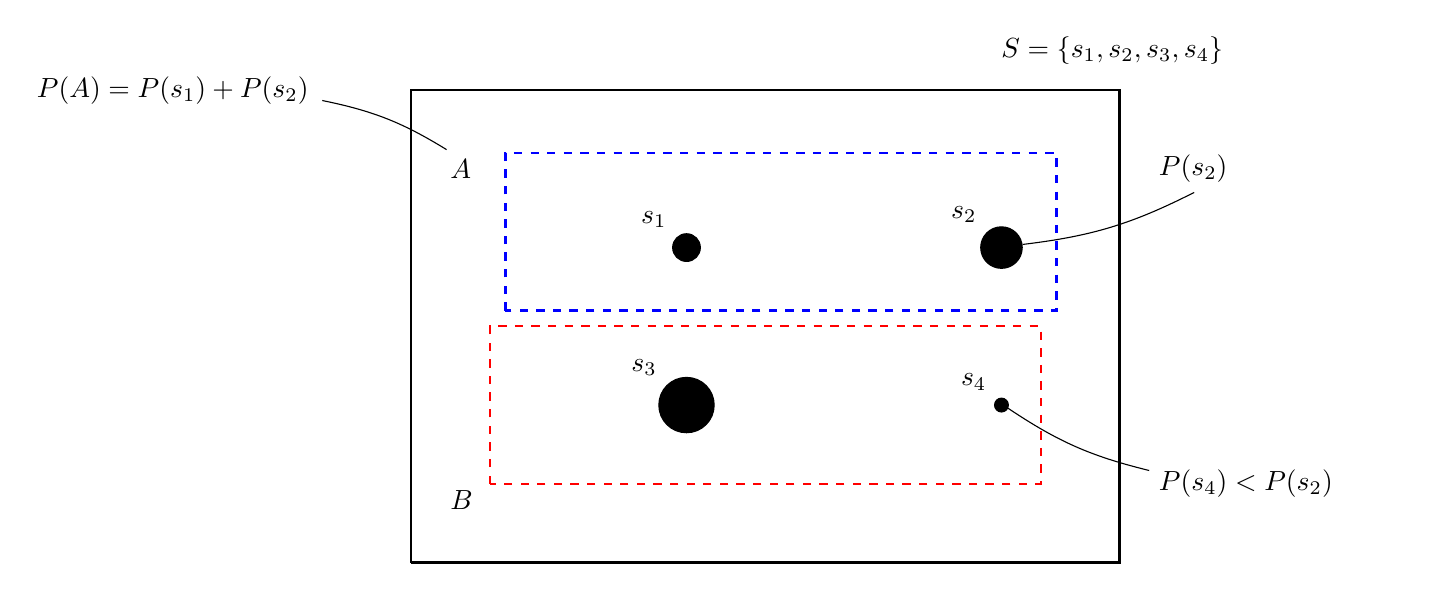
\begin{tikzpicture}[scale=1]
\draw[thick]
(0,0) coordinate --
(0,6) coordinate --
(9,6) coordinate --
(9,0) coordinate --
(0,0) coordinate;

\draw[thick,dashed,red]
(1,1) coordinate --
(1,3) coordinate --
(8,3) coordinate --
(8,1) coordinate --
(1,1) coordinate;

\begin{scope}[xshift=0.2cm,yshift=0.2cm]
\draw[thick,dashed,blue]
(1,3) coordinate --
(1,5) coordinate --
(8,5) coordinate --
(8,3) coordinate --
(1,3) coordinate;
\end{scope}

\node[label=above left:{$s_1$},draw,fill=black,circle,inner sep=0pt,minimum size=10pt] at (3.5,4) {};
\node[label=above left:{$s_2$},draw,fill=black,circle,inner sep=0pt,minimum size=15pt] (s2) at (7.5,4) {};
\node[label=above left:{$s_3$},draw,fill=black,circle,inner sep=0pt,minimum size=20pt] at (3.5,2) {};
\node[label=above left:{$s_4$},draw,fill=black,circle,inner sep=0pt,minimum size=5pt] (s4) at (7.5,2) {};

\node[text width=3cm] at (9,6.5) {$S = \{s_1,s_2,s_3,s_4\}$};
\node[text width=1cm] (A) at (1,5) {$A$};
\begin{scope}[yshift=-0.2cm]
\node[text width=1cm] at (1,1) {$B$};
\end{scope}

\node[text width=2cm] (s2label) at (10.5,5){$P(s_{2})$};
\draw (s2) to [bend right=10] (s2label);

\node[text width=3cm] (s4label) at (11,1){$P(s_{4}) < P(s_{2})$};
\draw (s4) to [bend right=10] (s4label);

\node[text width=3.5cm] (Alabel) at (-3,6){$P(A)=P(s_1) + P(s_2)$};
\draw (A) to [bend right=10] (Alabel);

%\path[bend right=10] (s2) edge {} (s4);

\end{tikzpicture}
\end{document}